\documentclass[a4paper,11pt]{article}

%%%%%%%%%%%%%%%%%%%%%%%%%%%%%%%%%%%%%%%%%%%%%%%%%%%%%%%%%%%%%%%%%%%%%%%%
% Paquetes utilizados
%%%%%%%%%%%%%%%%%%%%%%%%%%%%%%%%%%%%%%%%%%%%%%%%%%%%%%%%%%%%%%%%%%%%%%%%

% Gráficos complejos
\usepackage{graphicx}
\usepackage{caption}
\usepackage{subcaption}
\usepackage{placeins}

% Soporte para el lenguaje español
\usepackage{textcomp}
\usepackage[utf8]{inputenc}
\usepackage[T1]{fontenc}
\DeclareUnicodeCharacter{B0}{\textdegree}
\usepackage[spanish]{babel}

% Código fuente embebido
\usepackage{listings}
\usepackage{courier}

% PDFs embebidos para el apéndice
\usepackage{pdfpages}

% Matemáticos
\usepackage{amssymb,amsmath}

% Tablas complejas
\usepackage{multirow}

% Formato de párrafo
\setlength{\parskip}{1ex plus 0.5ex minus 0.2ex}

% Subrayado de palabras
\usepackage[normalem]{ulem}

% Formato de listados de código
\lstset{
  basicstyle=\footnotesize\ttfamily,
  numberstyle=\tiny,
  numbersep=5pt,
  tabsize=2,
  extendedchars=true,
  breaklines=true,
  stringstyle=\color{white}\ttfamily,
  showspaces=false,
  showtabs=false,
  xleftmargin=17pt,
  framexleftmargin=17pt,
  framexrightmargin=5pt,
  framexbottommargin=4pt,
  showstringspaces=false,
  language=SQL
}
\usepackage{caption}
\DeclareCaptionFont{white}{\color{white}}
\DeclareCaptionFormat{listing}{\colorbox[cmyk]{0.43, 0.35, 0.35,0.01}{\parbox{\textwidth}{\hspace{15pt}#1#2#3}}}
\captionsetup[lstlisting]{format=listing,labelfont=white,textfont=white, singlelinecheck=false, margin=0pt, font={bf,footnotesize}}

%%%%%%%%%%%%%%%%%%%%%%%%%%%%%%%%%%%%%%%%%%%%%%%%%%%%%%%%%%%%%%%%%%%%%%%%
% Título
%%%%%%%%%%%%%%%%%%%%%%%%%%%%%%%%%%%%%%%%%%%%%%%%%%%%%%%%%%%%%%%%%%%%%%%%

% Título principal del documento.
\title{\textbf{Trabajo Práctico: Hiposoft}}

% Información sobre los autores.
\author{
  Gabriel Jaimerena,      \textit{P. XX.XXX}                      \\
  Lorena Kalaydjian,     \textit{P. XX.XXX}                      \\
  Sergio Matías Piano,     \textit{P. 85.191}                      \\
  Javier Daniel Zaniratto, \textit{P. 90.886}                      \\
  \\
  \normalsize{1do. Cuatrimestre de 2013}                           \\
  \normalsize{75.15 - Bases de datos}                              \\
  \normalsize{Facultad de Ingeniería, Universidad de Buenos Aires}
}
\date{}

%%%%%%%%%%%%%%%%%%%%%%%%%%%%%%%%%%%%%%%%%%%%%%%%%%%%%%%%%%%%%%%%%%%%%%%%
% Documento
%%%%%%%%%%%%%%%%%%%%%%%%%%%%%%%%%%%%%%%%%%%%%%%%%%%%%%%%%%%%%%%%%%%%%%%%

\begin{document}

% ----------------------------------------------------------------------
% Top matter
% ----------------------------------------------------------------------
\thispagestyle{empty}
\maketitle

\begin{abstract}

  Este informe resume el desarrollo del trabajo práctico de la materia Base
  de Datos (75.15) dictada en el segundo cuatrimestre de 2013 en la Facultad de
  Ingeniería de la Universidad de Buenos Aires. El mismo consiste en el
  modelado de datos de un software de cotización de pólizas de automotor y otros riesgos,
  cuyos requisitos fueron extraído de un caso de estudio real.

\end{abstract}

\clearpage

% ----------------------------------------------------------------------
% Tabla de contenidos
% ----------------------------------------------------------------------
\tableofcontents
\clearpage


% ----------------------------------------------------------------------
% Desarrollo
% ----------------------------------------------------------------------
\part{Desarrollo}


\section{Modelo de entidad-interrelación} \label{sec:der}

\subsection{Hipótesis}

\begin{enumerate}

  \item 
  
\end{enumerate}


\subsection{Diagrama de entidad-interrelación}

 En la figura \ref{fig:der} se incluye el diagrama de entidad-interrelación
 final desarrollado para representar el dominio modelado cuyo relevamiento se
 detalla en el enunciado.

\begin{figure}[h!t]
  \centering
  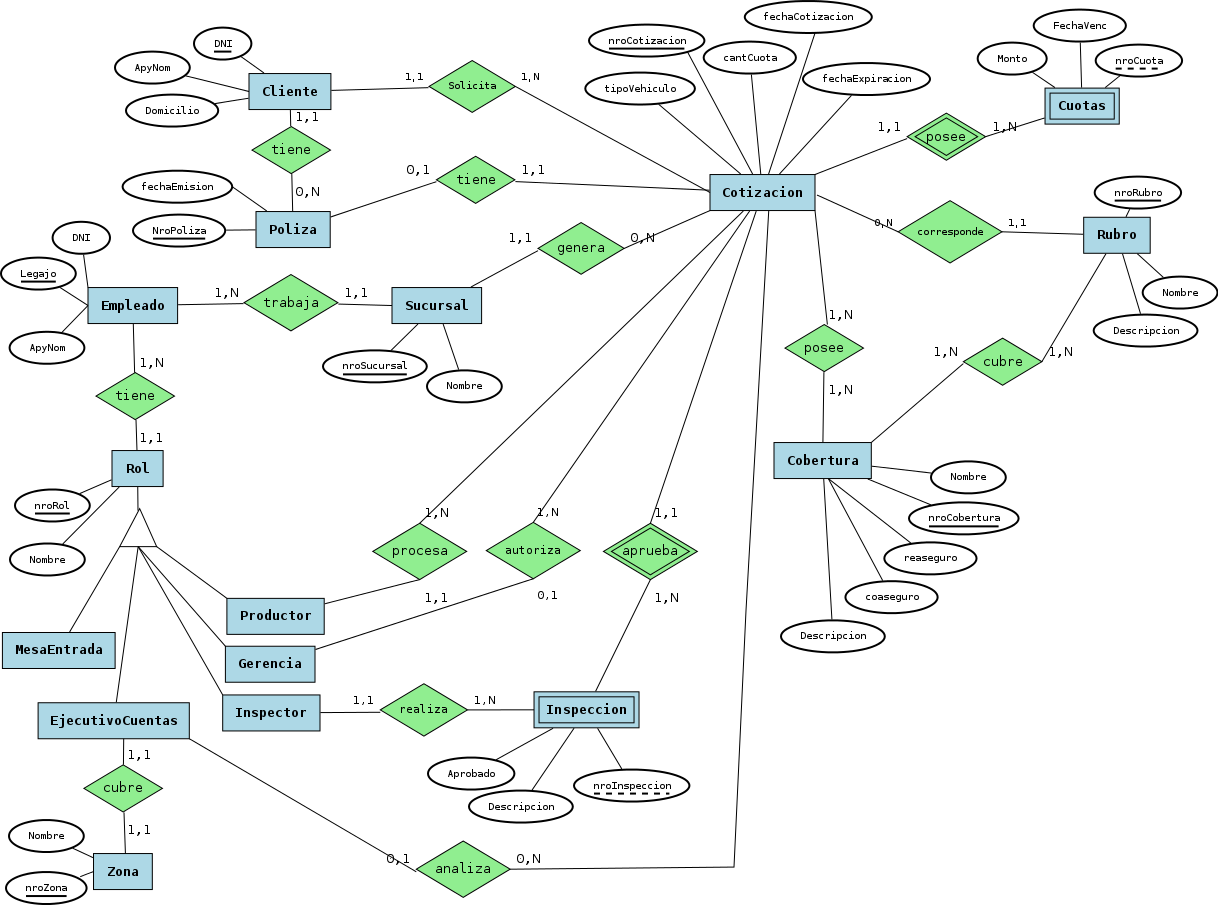
\includegraphics[width=1.5\textwidth, angle=90]{build/images/der.png}
  \caption{Diagrama de entidad-interrelación} \label{fig:der}
\end{figure}

\FloatBarrier


\subsection{Restricciones adicionales}

% Las siguientes restricciones adicionales se detallan a continuación por
% pertenecer al modelo de entidad-interrelación. No están representadas en el
% diagrama dado que su inclusión agregaba complejidad adicional sobre en la
% figura que consideramos innecesaria.

\begin{enumerate}

  \item 
  
\end{enumerate}

\section{Diccionario de datos}

\subsection{Cliente}

Representa las distintas personas físicas que solicitarán cotizaciones para asegurar 
a sus distintos vehículos.

\begin{itemize}

  \item \textbf{\uline{DNI}} Clave que identifica a un cliente.
  
  \item \textbf{Apellidos} Apellidos del cliente.

  \item \textbf{Nombres} Nombres del cliente.
  
  \item \textbf{Domicilio} Lugar donde reside el cliente.
  
\end{itemize}

\subsection{Cotizacion}

Representa las distintas formas de asegurar un vehículo que  que los clientes recibirán para poder asegurar
un vehículo.

\begin{itemize}

  \item \textbf{\uline{IdCotizacion}} Número único e identificatorio de cada cotización.
  
  \item \textbf{TipoVehiculo} Almacena el tipo de vehículo para el cual la cotización ha sido generada.

  \item \textbf{FechaExpiracion} Fecha en la cual deja de tener validez ésta cotización.
    
\end{itemize}

\subsection{Plan de pago}

Indica la forma en la que se deberá efectuar los pagos de las distintas cotizaciones.

\begin{itemize}

  \item \textbf{\dashuline{IdPlan}} Número que identifica cada plan de pago.

  \item \textbf{\dashuline{NroCuota}} Número de cuota del pago.
    
  \item \textbf{\uline{IdCotizacion}} Número único e identificatorio de cada cotización.
  
  \item \textbf{Monto} Suma de dinero que se deberá pagar en una determinada cuota.

  \item \textbf{FechaVencimiento} Fecha hasta la cual se puede realizar el pago.
  
  \item \textbf{CantCuota} Cantidad de cuotas.
    
\end{itemize}

\subsection{Póliza}

Los distintos seguros que contrató cada cliente.

\begin{itemize}
   
  \item \textbf{\uline{NroPoliza}} Número único e identificatorio de cada póliza.
      
\end{itemize}

\subsection{Sucursal}

Las distintas sucursales en las que los clientes podrán solicitar cotizaciones para asegurar sus vehículos

\begin{itemize}
   
  \item \textbf{\uline{IdSucursal}} Número que identifica a una sucursal.
  
  \item \textbf{Nombre} Nombre de la sucursal.
  
\end{itemize}

\subsection{Empleado}

Representa los trabajadores que realizarán las tareas necesarias para generarle cotizaciones
a los distintos clientes.

\begin{itemize}
   
  \item \textbf{\uline{Legajo}} Número interno que representa a cada empleado.
  
  \item \textbf{DNI} Documento de indentidad del empleado.
  
  \item \textbf{Nombres} Nombre del empleado.
  
  \item \textbf{Apellidos} Apellidos del empleado.
  
\end{itemize}

\subsection{Rol}

Representa los distintos puestos de trabajo en el que un empleado puede trabajar.

\begin{itemize}
   
  \item \textbf{\uline{IdRol}} Número identificatorio de cada rol.
  
  \item \textbf{Nombre} Nombre descriptivo del rol.
  
\end{itemize}

\subsubsection{Mesa de entradas}

Representa a los empleados que recibirán las solicitudes para asegurar.

\subsubsection{Ejecutivo de cuenta}

Empleados que analizarán en casos especiales las cotizaciones.

\subsubsection{Productor}

Empleados que procesarán las distintas cotizaciones.

\subsubsection{Gerencia}

Empleados que autorizarán las distintas cotizaciones.

\subsubsection{Inspector}

Empleados que realizarán inspecciones para determinar 
la aprobación o no de las cotizaciones.

\subsection{Inspección}

Las distintas visitas al vehículo de los inspectores para la 
aprobación de las cotizaciones

\begin{itemize}
   
  \item \textbf{\dashuline{IdInspeccion}} Número identificatorio de cada inspección.
  
  \item \textbf{Aprobado} Guarda si fue aprobada la cotización.
  
  \item \textbf{Descripcion} Almacena el por qué de la aprobación o no de la cotización.
  
\end{itemize}

\subsection{Zona}

Son las distintas zonas que cubrirán los ejecutivos de cuenta.

\begin{itemize}
   
  \item \textbf{\uline{IdZona}} Número identificatorio de cada zona.
  
  \item \textbf{Nombre} Nombre descriptivo de la zona.
  
\end{itemize}

\section{Modelo relacional}

\subsection{Diagrama relacional}

% En la figura \ref{fig:relacional} se incluye un diagrama representativo del
% modelo relacional desarrollado para el modelo de entidad-interrelación
% detallado en la sección \ref{sec:der}.

\begin{figure}[h!t]
%  \centering
%  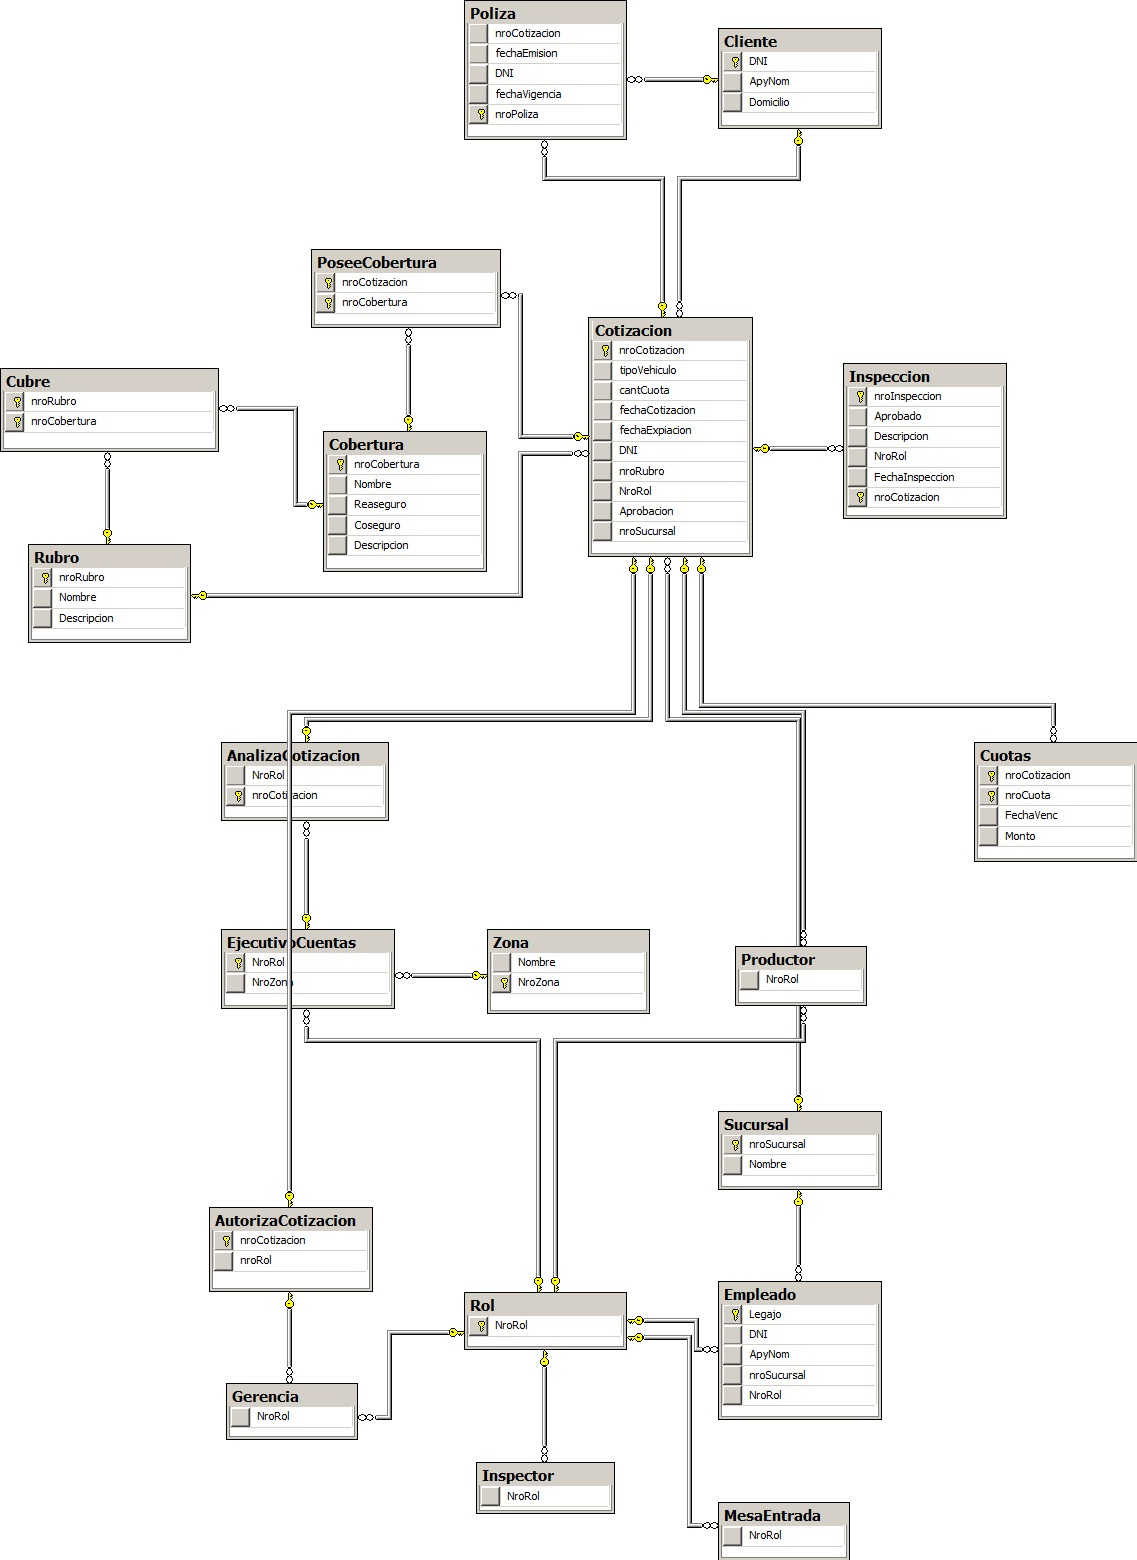
\includegraphics[width=1.65\textwidth, angle=90]{build/images/rel.png}
%  \caption{Modelo relacional} \label{fig:relacional}
\end{figure}

\FloatBarrier

\subsection{Scripts de creación}

%A continuación se incluyen los scripts de creación de las tablas del modelo
%relacional para ser ejecutado en un sistema de bases de datos que interprete
%SQL, particularmente las instrucciones DDL de dicho lenguaje. No se incluyen
%las instrucciones, normalmente específicas al motor propiamente dicho, de
%creación de usuarios, roles, schemas y bases de datos correspondientes.

%\lstinputlisting{sql/schema.sql}

\clearpage

\part{Apéndice}
\appendix

\section{Enunciado original}\label{sec:enunciado}
\includepdf[pages={-}, frame=true, pagecommand={}, noautoscale=true, scale=0.7]{doc/enunciado.pdf}

\end{document}

